\section{The Charm Gateway}
\label{sec:gateway}

% {\color{blue} Points to cover
% \begin{itemize}
%     \item Hardware + block diagram + capability + how to decode IQ streams
%     \item Local detection algorithm
%     \item Optional: (LoRa-aware) compression
% \end{itemize}

% }

We first describe Charm's design at the gateway to enable accurate decoding of
weak clients, by relaying suspected weak signals to the cloud. Charm achieves
this first through a software algorithm at the gateway that identifies weak
transmissions that may be significantly below the noise floor. We further
implement this approach in hardware by building a custom programmable radio
platform for the gateway, that streams and processes raw I/Q samples using an
FPGA. We show how a Charm-gateway can detect weak signals in real-time through
this design, while simultaneously being programmable and responding to policy
changes from the cloud.

\subsection{Locally Detecting Weak Signals}
\label{sec:local-detection}

To reap the benefits of coherent diversity combining across multiple gateways,
Charm must relay weak signals to the cloud. Yet,
uploading all received signals to overcome this problem is
unfeasible given that gateways have limited uplink bandwidth to the cloud. To
put this in perspective, streaming all received I/Q samples to the cloud
requires an uplink bandwidth of 72 Mbps. However, the vast
majority of LPWAN gateways are likely to be user-deployed hardware such as
set-top boxes that cannot afford this bandwidth. Indeed, this creates
trade-off between detecting weak transmitters and conserving uplink
bandwidth.

Charm breaks this trade-off by detecting weak signals well below the noise
floor at a single LoRaWAN gateway. At a high level, our solution relies on the
structure of the LoRa protocol. Specifically, LoRa transmits signals in
the form of chirps, i.e. signals whose frequencies increase linearly in time.
In addition, several of these chirps are identical. For instance, consider the
initial preamble  in LoRaWAN with as many as 16 identical and consecutive
chirps. This means one can design a receiver that coherently sums up adjacent
symbols of any received signal over a sliding window. If the summing-up
operation is truly coherent, the underlying signal (i.e. the chirp) will add
up constructively, while noise will add up incoherently. In effect, this
boosts the signal-to-noise ratio of the received signal significantly,
allowing us to detect at least the preamble of a LoRaWAN packet. One can then
deliver a long chunk of packets surrounding this preamble to the cloud.

However the resolution of the above approach is a function of preamble length
-- the longer the preamble sequence is, the greater will be the extent of
noise that Charm can tolerate. Transmitting extremely long preambles increases
the overhead of the communication system, and in the long term, impacts
battery life. Charm therefore develops an approach that can detect weak
signals by leveraging data symbols in addition to the preamble -- even though
the transmitted data sequence is unknown a priori at the gateway. We detail
our approach below.

\noindent \textbf{Leveraging the structure of LoRaWAN data: } Charm seeks to
use the structure of the data symbols in LoRaWAN to improve detection of the
packet in the presence of noise. Indeed, much akin to the preamble, the data
symbols of a LoRaWAN packet are also composed of a sequence of chirps. Unlike
the preamble though, LoRaWAN data is composed of a sequence of chirps with
different frequency-shifts based on the bits they represent. Assuming that the
underlying data in a message is completely unknown and arbitrary, this makes
looking for structure within the data challenging.


\begin{figure}
    \centering
    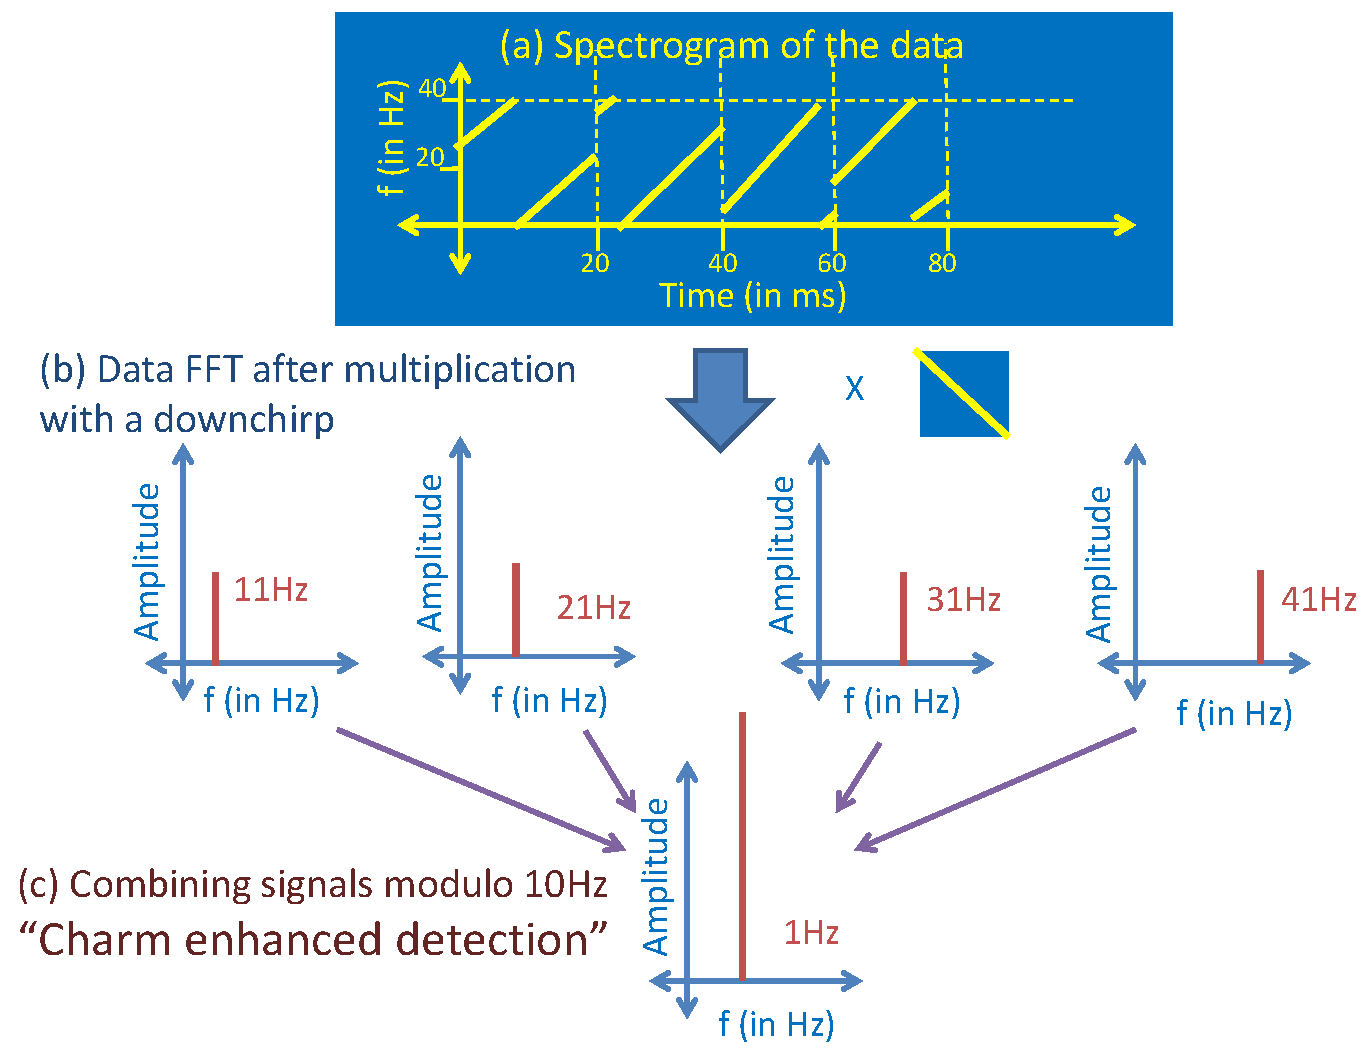
\includegraphics[width=0.85\columnwidth]{figures/CharmEnhancedDetection_cropped}
        \vspace*{-0.1in}
    \caption{The enhanced Charm packet detection process: The chirp signal (a)
    is multiplied by a downchirp in the Fourier domain (b). Windows of the
    resulting signal are then combined together (c) for threshold detection.}
    \label{fig:enhanced_charm}
    \compactimg
\end{figure}

Charm relies on the fact that while the data does cause shifts in frequencies
of chirps within the packet -- these shifts are not completely random. In
particular, chirps can undergo a discrete number of possible shifts based on
the number of bits per chirp. For a spreading factor of $SF$ (i.e. a
transmission data rate of $SF$ bits per chirp), the frequency shift is one of
$2^{SF}$ values. Charm therefore implements a solution that coherently
reinforces adjacent chirps, modulo the minimum possible frequency shift
between them. This ensures that regardless of their underlying data, adjacent
chirps always add up to reinforce each other while noise adds up destructively
as before. Given that there are a significantly larger number of data symbols
when compared to preamble symbols in any transmission, this provides an
additional mechanism to detect packets below the noise.

Mathematically, let $y_1, y_2, \dots, y_m$ denote the $m$ received data
symbols and $x_1, x_2, \dots, x_m$ denote the transmitted data bits encoded as
frequency shifts, each a number between $0$ and $2^{SF-1}$ where $SF$ is the
spreading factor. Let $\delta f = \text{Bandwidth} / 2^{SF}$ denote the
minimum possible frequency separation between two encoded data chirps.  Then
we can write the received signal at any time $t$ of the $i^{\text{th}}$ symbol
as:
\begin{align}
    y_i(t) = h e^{j 2 \pi (f(t) - x_i \delta f) t} + n_1 \label{eqn:yi}
\end{align}
Where $f(t)$ denotes the time varying frequency of the chirp, $j$ is the
square root of $-1$, $h$ represents the wireless channel and $n_i$ represents
noise.

When multiplied by $e^{-j 2 \pi f(t) t}$ and viewed in the Fourier domain,
this results in a single tone at frequency $x_i \delta f$ subject to noise.
Clearly the location of the tone is a function of the underlying data -- a
different quantity for different data symbols.

In contrast, let us sub-sample the above equation at times $t$ that are
multiples of $1/\delta f$ (let's say $t = \frac{k}{\delta f}$ for integer
values of $k$).

\begin{align}
    y_i\left(t\right) = h e^{j 2 \pi (f(t) - x_i \delta f) \frac{k}{\delta f}} + n_1 = h e^{j 2 \pi f(t) t} + n_1\label{eqn:yi2}
\end{align}
This time, when multiplied by $e^{-j 2 \pi f(t) t}$ and viewed in the Fourier
domain, this results in a single tone at frequency $0$ (subject to noise)
regardless of the underlying data in each symbol. In other words, sub-sampling
in the time domain led to aliasing of all the data peaks in the frequency
domain into one frequency bin (in this case, the DC bin), while noise is
smeared uniformly across all bins. Indeed, Charm repeats the sub-sampling
across multiple time steps separated  by $\frac{1}{\delta f}$ and averages the
results. The resulting average reinforces peaks corresponding to all the data
symbols coherently in one Fourier frequency bin, while noise adds up
incoherently among all remaining bins. This leads us to a very natural LoRaWAN
packet-detection mechanism that applies this operation across different
sliding windows of the received signals. We signal the presence of a packet
once our algorithm detects a significant peak in the Fourier domain that
dominates other peaks (subject to a threshold). Given that our approach
averages results over a large number of data symbols, it remains resilient to
noise without making assumptions about the contents of the packet itself.

\RestyleAlgo{boxruled}
\LinesNumbered
\begin{algorithm}[ht]
\caption{Charm's enhanced detection algorithm}
\label{alg:algorithm-label2}
 \For{bits in instream}{
 [C=I+jQ]=downsample(bits)\;
 \For{chirp\_length in C}{
    F=chirp\_length$*$down\_chirp\;
    FCollect.collect(F)\tcp*{Data Collection} 
 }
 C=FCollect.modulo($\delta f$)\tcp*{Modulus Bucketing}
 \If{$\frac{max(abs(fft(C)))}{mean(abs(fft(C)))}>\tau$}{
    SEND C to CLOUD \tcp*{Packet Forwarding}
 }
 }
\end{algorithm}

\noindent \textbf{Mitigating Frequency Offsets: } To add up signals from
adjacent symbols coherently, Charm must assume that the received symbols in
these signals are identical -- subject to noise and discrete shifts in
frequency due to the data (as described above). In practice however, wireless
signals from the LPWAN client to the gateway experiences an additional
arbitrary shift in frequency due to Carrier Frequency Offset (CFO). CFO stems
from the subtle variation in frequency between the clocks on the transmitter
and receiver. Given that the client is inexpensive, its clock often exhibits
large and arbitrary frequency differences relative to the gateway.
Additionally, the CFO for a given transmission received at different gateways
is also different and must be resolved individually.

Two properties of CFO make its impact on Charm's algorithm above particularly
damaging: (1) CFO unlike data introduces a frequency shift that is not
discrete, but continuous. As a result, it is not simply eliminated by looking at
the chirp in the Fourier domain ``modulo $\delta f$''  akin to the data as
described above. (2) CFO introduces a continuous phase shift $2 \pi
\Delta f_{CFO} t$ onto the received signal that accumulates over time. This
means that even otherwise identical received symbols may add up incoherently
owing to a time-varying phase shift.

The straw man approach to eliminate CFO would be an attempt to directly
estimate it. For instance, one could rely on the repeated symbols of the
preamble where any phase variation is purely a function of CFO. In particular,
the phase shift between two otherwise identical preamble symbols separated by
$t$ is simply $2 \pi \Delta f_{CFO} t$, which one can solve for to estimate $\Delta
f_{CFO}$ and eliminate its effect. However, this solution fails if the number of preamble symbols in the transmitted signal is insufficient to overcome noise. Further, this approach cannot exploit data symbols to estimate CFO, which, as explained earlier, are greater in number and would greatly enhance resilience to noise.

Charm overcomes this problem by realizing that while estimating $\Delta
f_{CFO}$ from the data symbols alone is challenging, it is sufficient to
estimate $\Delta f_{CFO}$ modulo $\delta f$ to detect the LoRa packet. To see
why, recall that the frequency offset over a packet $\Delta f_{CFO}$ can be
decoupled into two components: $[\frac{\Delta f_{CFO}}{\delta f}]\delta f + \{\frac{\Delta f_{CFO}}{\delta f}\}\delta f$, an
integer multiple of $\delta f$ and the remaining fractional component
respectively. When looking at the data chirps in the frequency domain modulo
$\delta f$, all the data symbols appear identical given that all frequency
shifts of the data are all multiples of $\delta f$. Similarly, the first term of the CFO:
$[\frac{\Delta f_{CFO}}{\delta f}]\delta f$ is also an integer multiple of $\delta f$ and therefore disappears under the modulo. Only the fractional part of the CFO: $\{\frac{\Delta f_{CFO}}{\delta f}\}\delta f$ persists
and introduces a time varying phase shift of $2 \pi \{\frac{\Delta f_{CFO}}{\delta f}\}\delta f t$
across symbols. This means that we can simply solve for the fractional component of CFO and eliminate its effect akin to the straw man approach, but using the data
symbols in the frequency domain modulo $\delta f$. In other words, Charm's
solution remains resilient to frequency offset, both in detecting the preamble
as well as data symbols of a LoRaWAN packet.

\subsection{Programmable Hardware Design}
\label{sec:hardware}

Charm must process raw I/Q samples from the gateway and selectively relay this
information to the cloud in real-time. However, existing LoRaWAN gateway
hardware cannot provide the raw I/Q streams necessary for joint decoding. In
contrast, deploying a full software-defined radio (SDR) at the gateway allows
packet decoding, it comes with high cost in term of power, sensitivity and
unit price. We therefore develop a custom Charm hardware platform shown in
\figref{lpran-hardware-images} as an auxiliary peripheral to a gateway and can
provide the necessary quadrature streams. Key to our performance is a
light-weight, low-cost and easy-to-reprogram hardware accelerator for data
reduction enabling further local processing (e.g. on the accelerator or by a
Raspberry Pi). In effect, we allow for a system that simultaneously allows
some SDR-like programmability of the PHY while maintaining high performance
and low cost.

\noindent  {\bf Compressing the Data Stream: } The raw IQ stream would be too
much for a low-power microprocessor, and  also contain too much redundant
information for our purpose. In particular, we use the SX1257 RF front-end
that provides 1-bit delta-sigma modulated signals at a whopping 36 MSps each
for the I and Q streams.  In order to keep the data stream to a more
microprocessor-friendly load, the design would require some lossless
compression. Through careful choice of parameters, we chose to compress the IQ
stream by summing consecutive samples in windows of size 64 and convert it
into a single 7-bit sample:
\begin{equation}
x_i = \sum_{j=64*i}^{64*i + 63} s_j
\end{equation}
, where ($x_i$) is the analyzable samples, and ($s_j$) is the I/Q sample
rates. A window size of 64 is selected since we are only interested in a final
bandwidth of approximately 500 kHz that the RF front-end is capable of
capturing. Upon applying the above technique, the compressed I/Q streams
generate data at a rate of 9 Mbps, down from the original 72 Mbps.

\begin{figure}[t]
\centering
\begin{tabular}{@{}c@{}}
\subfloat[Block diagram of the Charm programmable radio hardware platform]{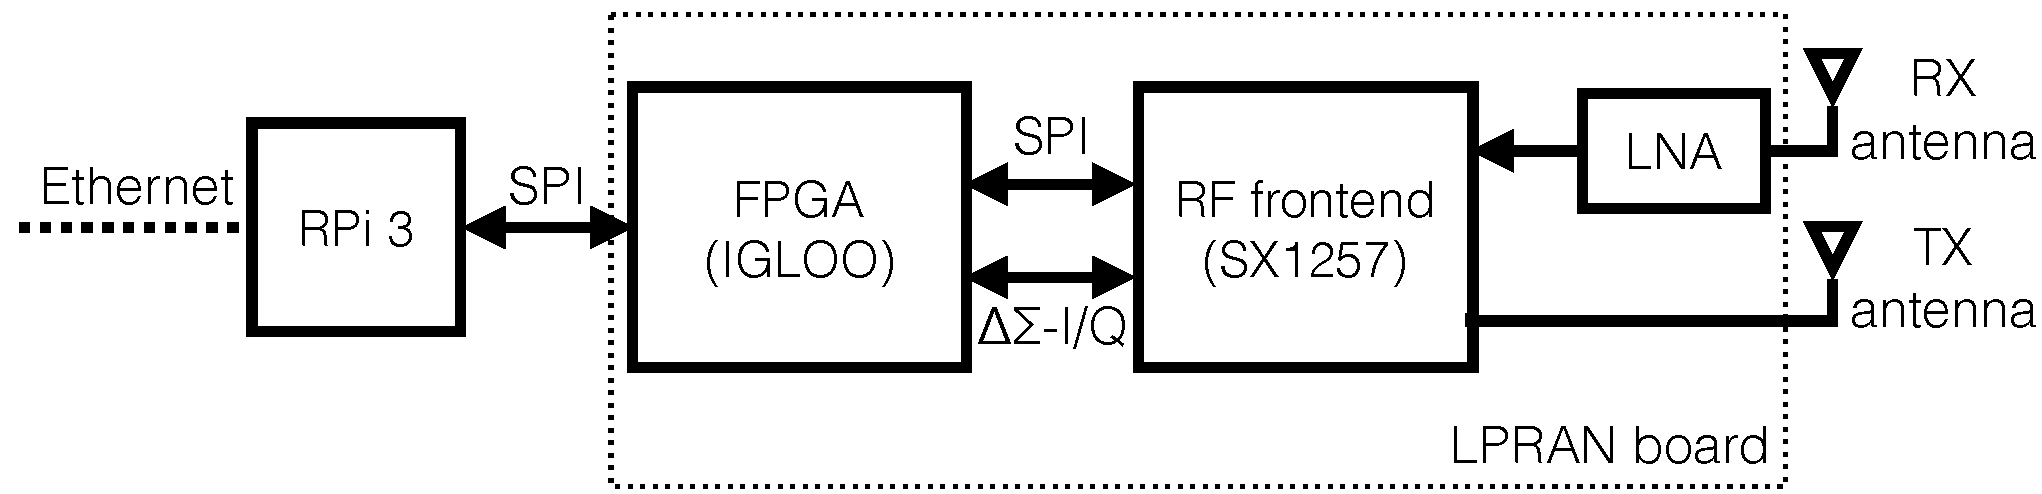
\includegraphics[width=0.40\textwidth]{figures/lpran-block_cropped}
\label{fig:lpran-block}} \\
\subfloat[Charm programmable gateway]{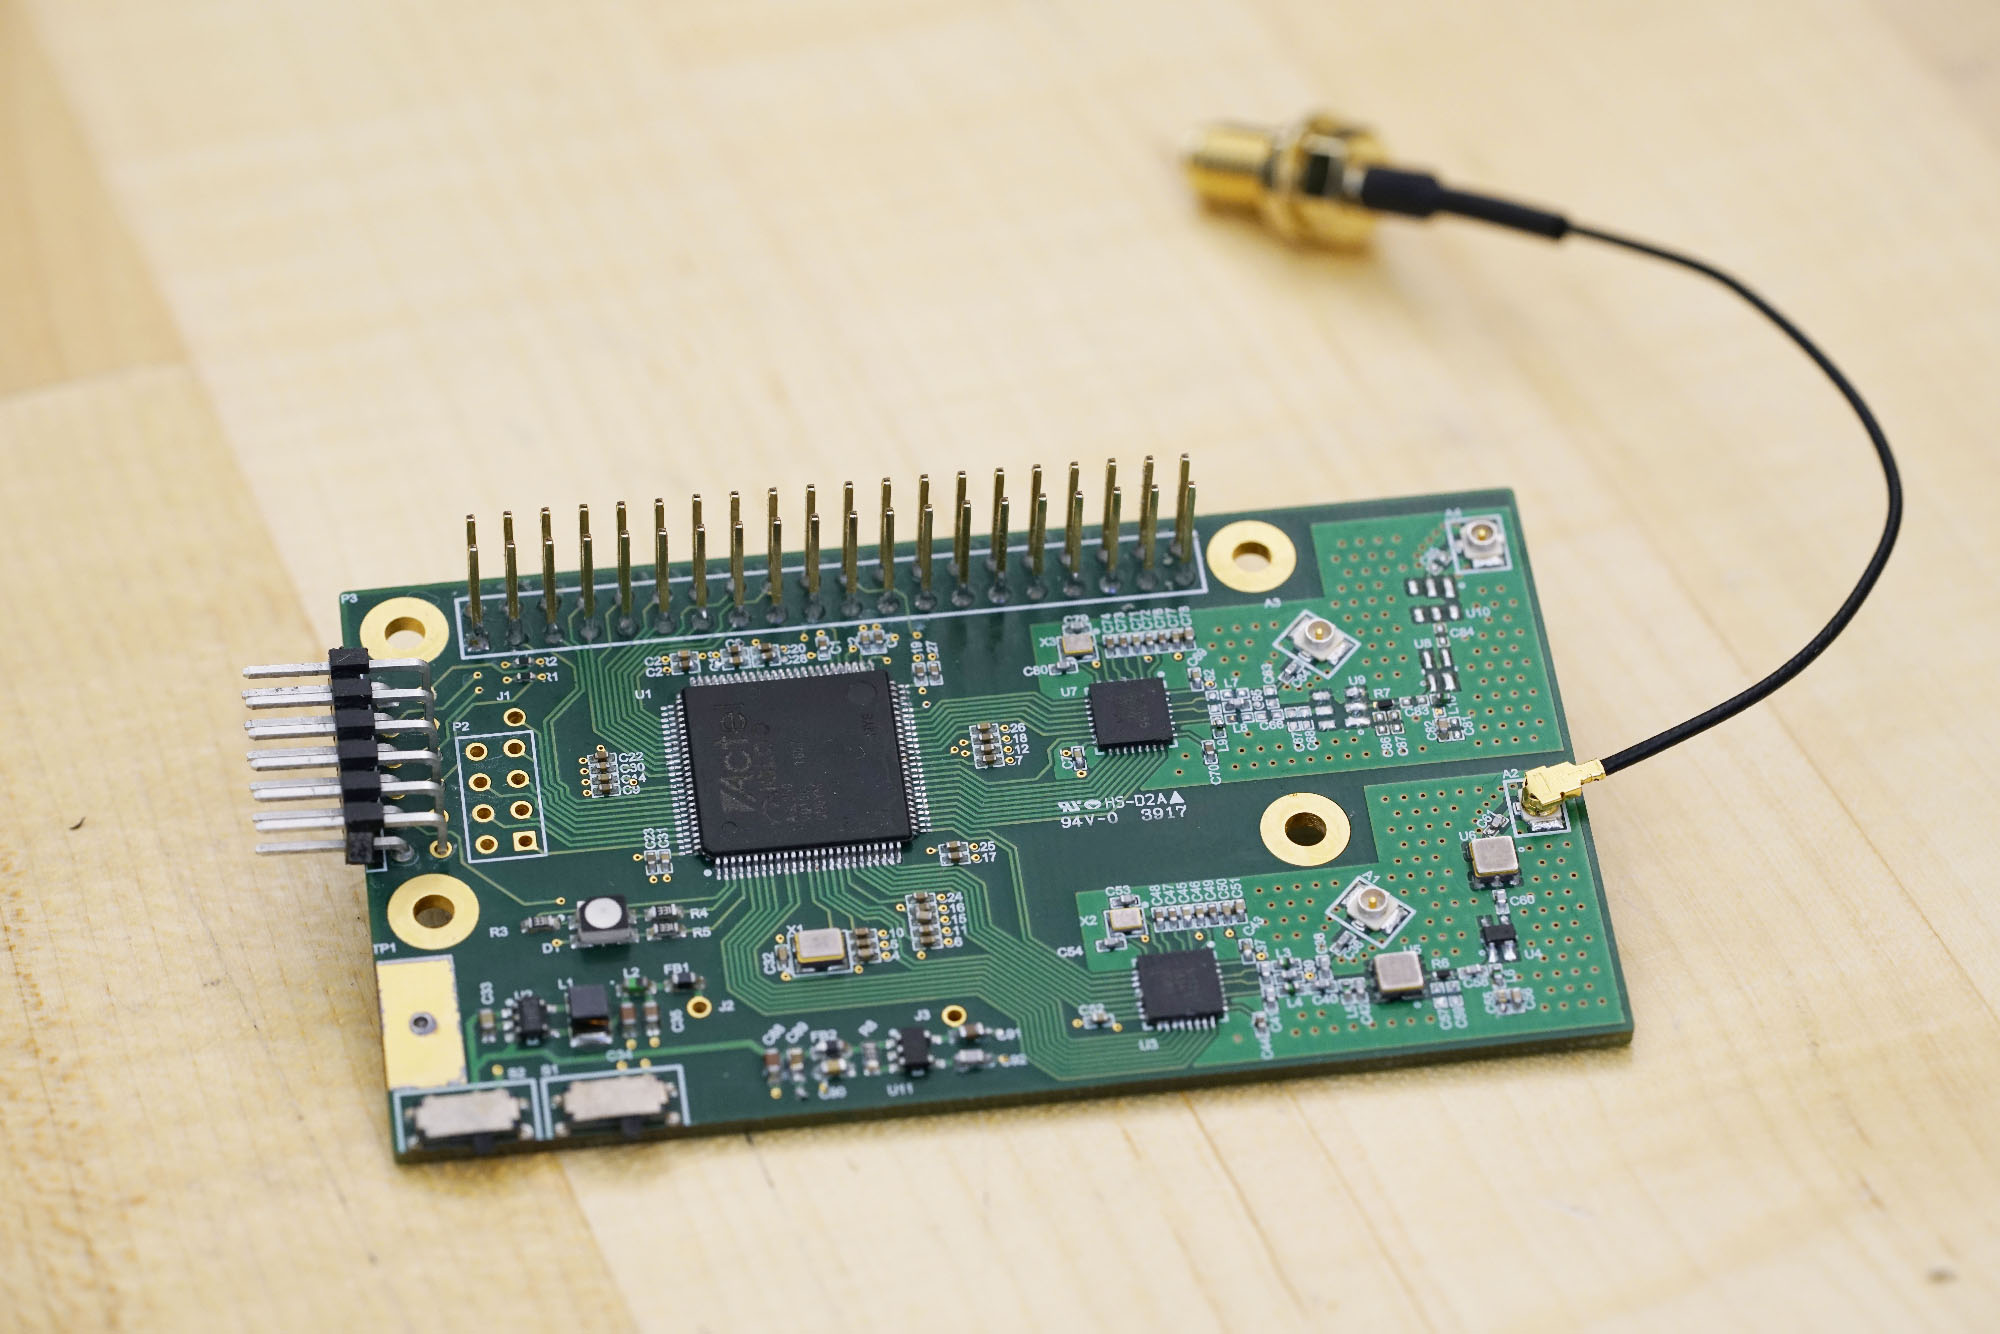
\includegraphics[width=0.23\textwidth, height=1.2in]{figures/gw-anon-sm}
\label{fig:gw-pcb}} 
\subfloat[Gateway with Charm hardware and LoRaWAN~concentrator]{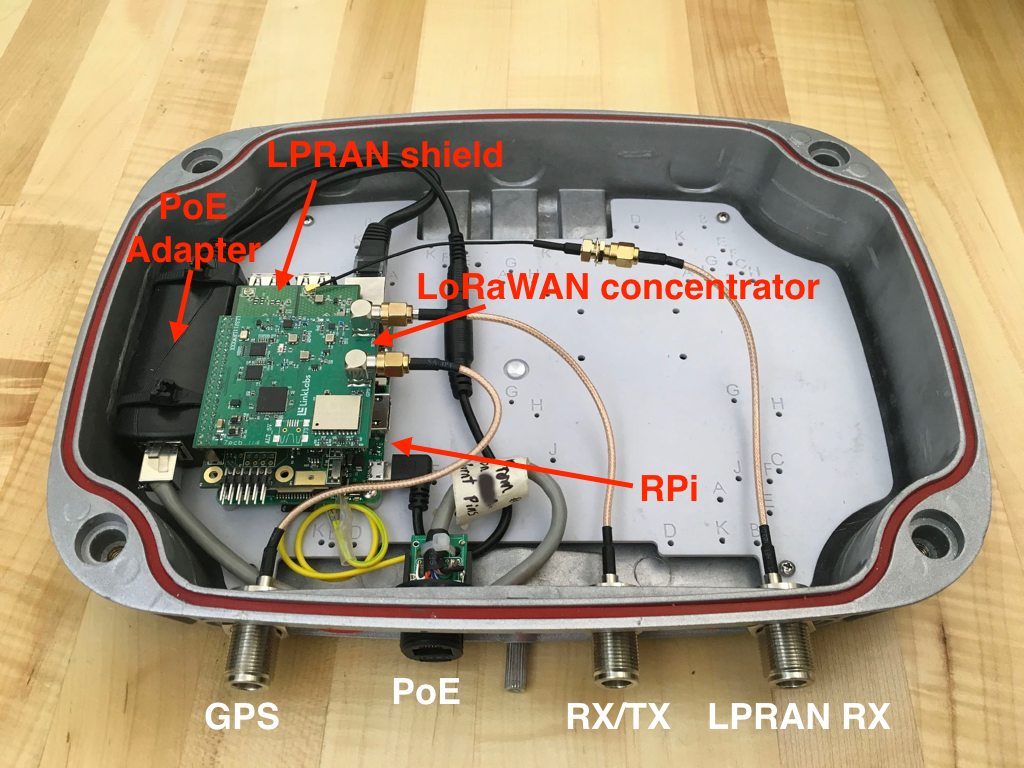
\includegraphics[width=0.23\textwidth, height=1.2in]{figures/annotated_gateway}
\label{fig:gw-annotated}}
\end{tabular}
\vspace*{-0.1in}
\caption{Charm Hardware Platform}
\label{fig:lpran-hardware-images}
\compactimg
\end{figure}

\noindent  {\bf Programmability: } The delta-sigma I/Q samples are processed
locally on a Microsemi IGLOO AGL250 FPGA, which performs the necessary
compression for data reduction.   The stream of data is transferred using a
high-speed serial interface (SPI) to the microprocessor (Raspberry Pi), and
forwarded when requested by the joint-decoder for additional processing. Each
block of samples are double buffered to ensure the validity of the data during
transfers. The microprocessor can then perform additional local processing,
time-stamping and temporary local storage until a stream is requested by the
joint-decoder. While our hardware platform is not a full-scale SDR, the FPGA
allows programmers to implement advanced real-time algorithms for packet
decoding and/or full duplex transmission across multiple channels. In
addition, the Raspberry Pi allows for ease of programmability when gathering
low-rate statistics about the received signals at the gateway. Overall, we
believe the Charm hardware platform will reduce the barrier for LPWAN
PHY-layer innovation for programmers and researchers across the board.